\setcounter{chapter}{4}

\chapter{导数的应用}

\section{函数的极值与最值}

{\bf 问题:}给定一个函数,如何求其最大和最小值?

{\bf P224-例1:}画出函数$f(x)=3x^4-4x^3-12x^2+3$在区间$[-2,3]$,通过
观察求其最大和最小值。

\begin{center}
% 	\resizebox{!}{4cm}{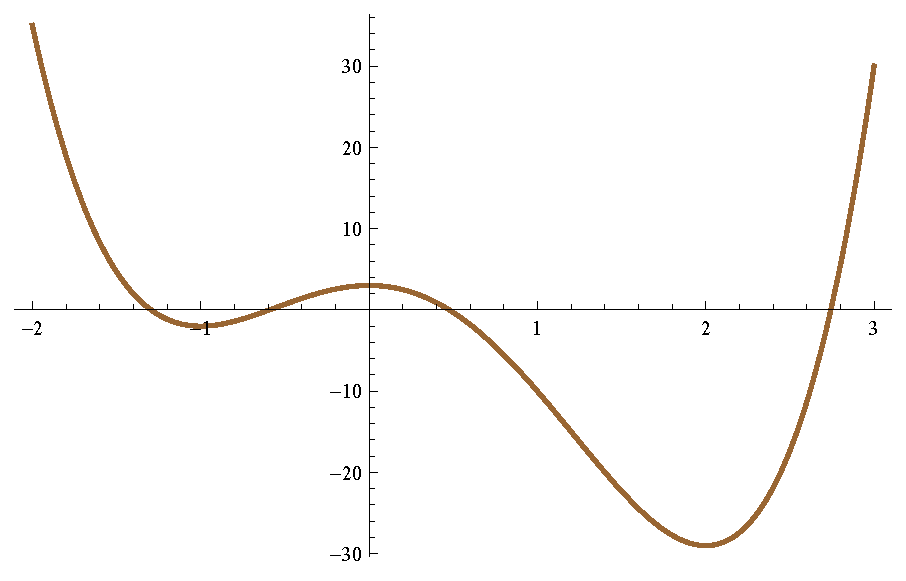
\includegraphics{./images/ch5/fmm_ori.pdf}}
	\resizebox{!}{5cm}{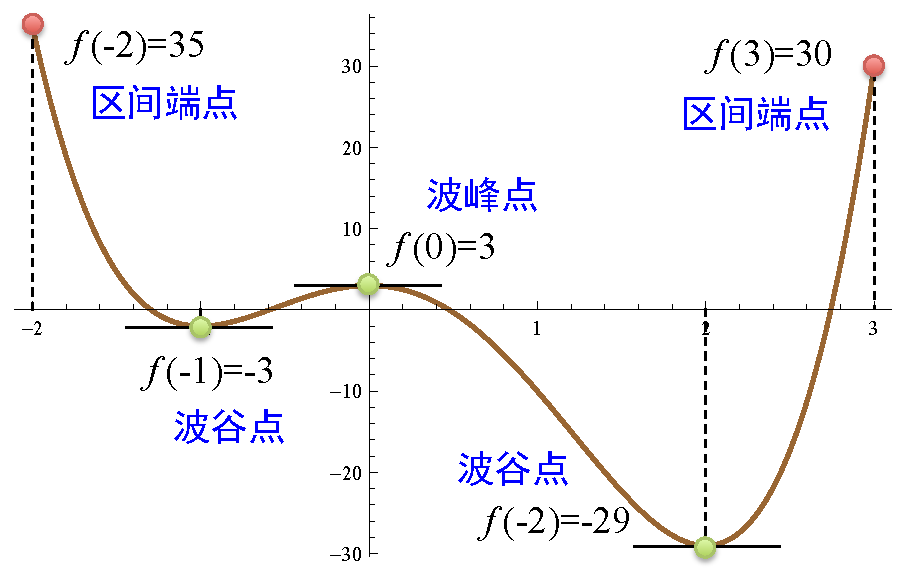
\includegraphics{./images/ch5/fmm_pt.pdf}}
\end{center}
\vspace{-2em}
$$f(-2)=35,\quad f(3)=30,\quad f(2)=-29$$

{\bf 定理5.1.1}(Fermat引理):若函数$f(x)$在$x_0$处可导,且在$x_0$的某邻域内,有
$$f(x)\geq f(x_0)\quad (\mbox{或}\quad f(x)\leq f(x_0))$$
则$f\,'(x_0)=0$。

\begin{shaded}
{\bf Fermat}:
% \resizebox{!}{3cm}{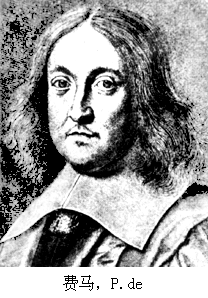
\includegraphics{./images/ch5/Fermat.png}}
{\it the prince of amateurs}

{\bf Fermat大定理:}
$n>2$时,方程$x^n+y^n=z^n$没有整数解
\end{shaded}

\subsection{极值}

{\bf 定义5.1.1:}设在$x_0$的某去心邻域内,恒有
$$f(x)<f(x_0)\quad (\mbox{或}\quad f(x)>f(x_0)),$$
则称$f(x_0)$是$f(x)$的一个{\it 极大(小)值},$x_0$称为$f(x)$的一个{\it 极值点}。

\begin{itemize}
  \setlength{\itemindent}{1cm}
  \item 函数在极值点处未必可导 
  \item 可导函数极值点处的导数为零 
  \item 导数为零的点({\it 驻点})未必是极值点
\end{itemize}

\begin{center}
	\resizebox{!}{4cm}{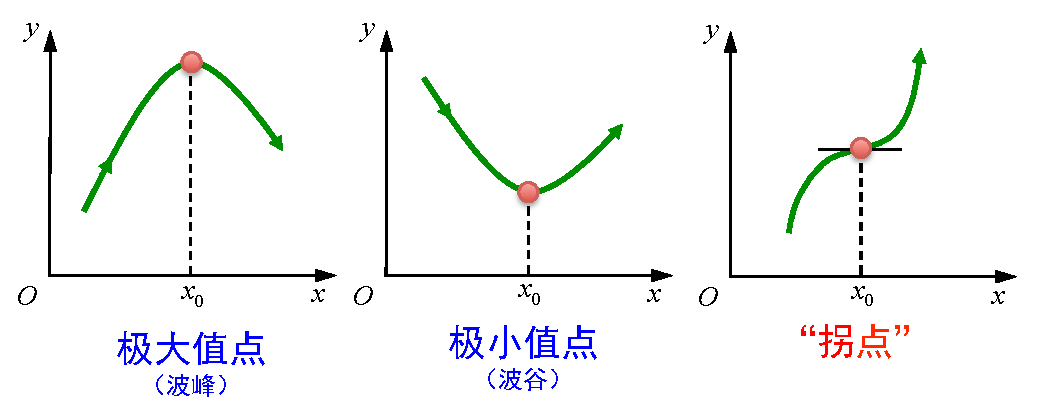
\includegraphics{./images/ch5/edge_pt.pdf}}
\end{center}

{\bf 定理5.1.2}(极值判定的充分条件)设$f(x)$在$x_0$附近连续,
若$f(x)$在$x_0$两侧单调性发生改变,则$f(x)$在$x_0$取极值。

{\bf 注:}连续函数单调性的分界点是函数的极值点。

{\bf 例:}判断正误
\begin{enumerate}[(1)]
  \setlength{\itemindent}{1cm}
  \item 函数的极大值一定是最大值\quad  ({$\times$}) 
  \item 函数的最大值一定是极大值\quad  ({$\times$}) 
  \item 函数的极大值一定比极小值大\quad  ({$\times$}) 
\end{enumerate}

\subsection{最值(最优化)问题}

{\bf 问:}在闭区间上,函数可能在什么位置取到最值?

\begin{center}
	\resizebox{!}{4cm}{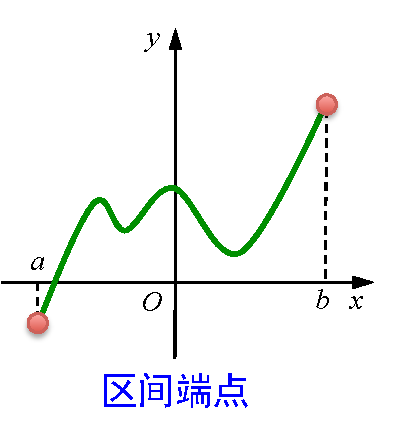
\includegraphics{./images/ch5/mm1.pdf}}
	\resizebox{!}{4cm}{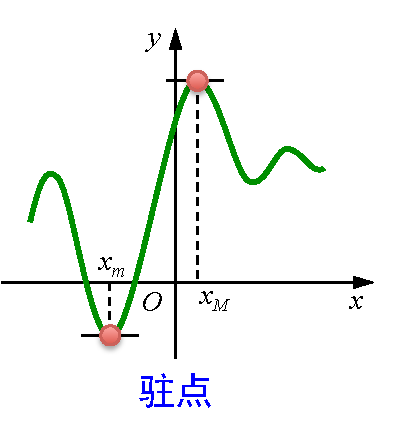
\includegraphics{./images/ch5/mm2.pdf}}
	\resizebox{!}{4cm}{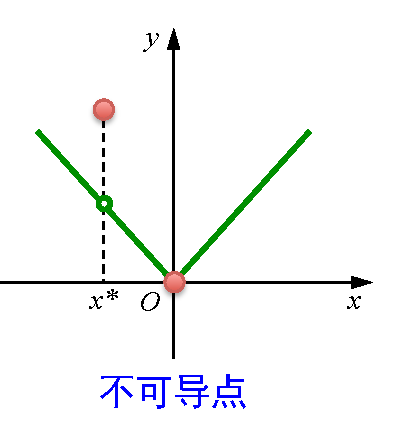
\includegraphics{./images/ch5/mm3.pdf}}
\end{center}

{\bf 求闭区间上连续函数的最值:}

\begin{enumerate}[(1)]
  \setlength{\itemindent}{1cm}
  \item 确定函数在区间内的所有{\it 驻点}和{\it 不可导点}$x_1,x_2,$ $\ldots,x_n$ 
  \item 逐个计算
  $f(a),f(x_1),f(x_2),\ldots,f(x_n),f(b)$,
  {\it 比较求得最大和最小值}。
\end{enumerate}

{\bf P224-例1:}求函数$f(x)=3x^4-4x^3-12x^2+3$在区间$[-2,3]$上的最大和最小值。

\begin{shaded}
{\bf 【最优化问题】}

{\bf 目标:}求函数$f(x)$的最大(小)值以及对应的最大(小)值点

{\bf 约束:}变量$x$满足一定的条件,例如:$x\in[a,b]$

\begin{itemize}
  \setlength{\itemindent}{1cm}
  \item 给定边长,求所能围成的矩形区域的最大面积? 
  \item 给定原材料,生产各种商品所能获得最大利润? 
  \item 为达到特定生产收益,所需投入的最少资源? 
  \item \ldots \ldots 
\end{itemize}

{\bf 解题过程:}
\begin{enumerate}[(1)]
  \setlength{\itemindent}{1cm}
  \item {\it 理解题意:}画图、定义变量 
  \item {\it 建立关系:}目标函数表达式 
  \item {\it 求解最值}
\end{enumerate}
\end{shaded}

{\bf P230-例5:}一个边长为$a$的方形铁皮,在四角各剪去一个边长为$x$的小正方形,然后折成
一个无盖的长方体容器,问当$x$取何值时,长方体容器的容积最大?

{\bf P230-例4:}用输油管连接离海岸12km的钻井平台和沿岸往下20km处的炼油厂。已知水下和陆上铺设
管道的成本分别是每公里50万元和30万元,问该如何设计线路,使总的建设成本最低?

\section{微分中值定理}

\subsection{Rolle定理}

{\bf 定理5.2.1:}若函数$f(x)$满足:
\begin{enumerate}[(1)]
  \setlength{\itemindent}{1cm}
  \item 在区间$[a,b]$上连续
  \item 在区间$(a,b)$内可导
  \item $f(a)=f(b)$
\end{enumerate}
则:存在$\xi\in(a,b)$,使得$f\,'(\xi)=0$。

{\bf 注:}三个条件缺一不可!!

{\bf 例:}证明:对函数$f(x)=(x-1)(x-2)(x-3)$,至少存在一点
$\xi\in(1,3)$,使得$f\,''(\xi)=0$。

{\bf 例}(Darboux定理)设$f(x)$在$[a,b]$上可导,且$f\,'_+(a)f\,'_-(b)<0$,
则存在$\xi\in(a,b)$,使得$f\,'(\xi)=0$。

{\bf 例:}设$f(x)$在$[a,b]$上满足Rolle定理条件,
且$f\,'_+(a)f\,'_-(b)>0$,则$f\,'(0)=0$在$(a,b)$内至少有两个根。

{\bf 例:}设$\df{a_0}{n+1}+\df{a_1}{n}+\ldots+a_n=0$,证明:方程
$$a_0x^n+a_1x^{n-1}+\ldots+a_n=0$$
在区间$(0,1)$内至少有一个根。

{\bf 推论}(Rolle定理的高阶推广)
设$f(x)$在$[x_0,x_n]$上有$n-1$阶连续导数,在$(x_0,x_n)$内
$n$阶可导,且
$$f(x_0)=f(x_1)=\ldots=f(x_n),\quad(x_0<x_1<\ldots<x_n),$$
则存在$\xi\in(x_0,x_n)$,使得$f^{(n)}(\xi)=0$。

\subsection{Lagrange中值定理}

{\bf 定理5.2.2:}若函数$f(x)$满足: 
\begin{enumerate}[(1)]
  \setlength{\itemindent}{1cm}
  \item 在区间$[a,b]$上连续 
  \item 在区间$(a,b)$内可导 
\end{enumerate}
则:存在$\xi\in(a,b)$,使得 
$$f\,'(\xi)=\df{f(b)-f(a)}{b-a}.$$

{\bf 推论(P237-例1)}导数恒为零的函数取值恒为常数。

{\bf 例:}设$\limx{+\infty}f(x)$和$\limx{+\infty}f\,'(x)$均存在,证明:
$$\limx{+\infty}f\,'(x)=0.$$

{\bf 例:}设$f(x)$在$U(x_0)$内连续,在$U^0(x_0)$内可导,
且$\limx{x_0}f\,'(x)=l$,则$$f\,'(x_0)=l.$$

{\bf 例:}证明:$\df{\ln x-\ln x_1}{x-x_1}<\df 1{x_1},\quad (0<x_1<x)$

{\bf 例:}设$f(x),g(x)\in C[a,b]$,在$(a,b)$内可导,且$f(a)=f(b)=0$,证明:存在
$\xi\in(a,b)$,使得:
$$f\,'(\xi)+f(\xi)g'(\xi)=0.$$
{\bf 注:}辅助函数的构造可以从不定积分中获得一些启发
\begin{itemize}
  \item {$y+\lambda y'=0$: $F(x)=e^{\lambda x}y$} 
  \item {$ny+xy'=0$: $F(x)=x^ny$} 
  \item {$f\,'(x)g(x)-f(x)g'(x)=0$: $F(x)=\df{f(x)}{g(x)}$}
\end{itemize}


{\bf P237-例2:}证明不等式:
$$\df{x}{1+x}<\ln(1+x),\;x>0$$

{\bf P237-例3:}证明方程$x^5+x-1=0$只有唯一实根。

{\bf P238-例4:}设$f(x)\in C[a,b]$,且$f(x)$在$(a,b)$内二阶可导,
连接函数曲线两端点的直线在$(a,b)$内至少与曲线存在一个交点,
则存在$\xi\in(a,b)$,使得$f\,''(\xi)=0$。

{\bf 思考:}若端点连线与函数曲线存在多个交点,能够得到什么结论?

\subsection{Cauchy中值定理}

{\bf 定理5.2.3:}若函数$f(x),\varphi(x)$满足: 
\begin{enumerate}[(1)]
  \setlength{\itemindent}{1cm}
  \item 在$[a,b]$上连续 
  \item 在$(a,b)$内可导,且$\varphi'(x)\ne 0$ 
\end{enumerate}
则:存在$\xi\in(a,b)$, 使得
$$\df{f(b)-f(a)}{\varphi(b)-\varphi(a)}=\df{f\,'(\xi)}{\varphi'(\xi)}$$

{\bf 注:}Cauchy中值定理可视为参数化的Lagrange中值定理

{\bf 例:}设$0<a<b$,$f(x)$在$[a,b]$上连续,在$(a,b)$内可导,证明:
\begin{enumerate}[(1)]
  \setlength{\itemindent}{1cm}
  \item 存在$\xi\in(a,b)$,使得:
	$$f(b)-f(a)=\ln\df ba\cdot \xi f\,'(\xi)$$
  \item 存在$\eta\in(a,b)$,使得:
    $$2\eta[f(b)-f(a)]=(b^2-a^2)f\,'(\eta)$$
\end{enumerate}

{\bf 例:}设$f(x)$在$[a,b]$连续,在$(a,b)$可导,且$a\geq 0$,则存在
$x_1,x_2,x_3\in(a,b)$,使得
$$f\,'(x_1)=(b+a)\df{f\,'(x_2)}{2x_2}=(a^2+ab+b^2)\df{f\,'(x_3)}{3x_3^2}$$

{\bf 注:}在使用中值定理前对要证明的等式进行必要的“整理”

{\bf 例:}设$f(x)$在$[a,b]$连续,在$(a,b)$可导,且$f\,'(x)\ne 0$,证明:
存在$\xi,\eta\in(a,b)$,使得
$$\df{f\,'(\xi)}{f\,(\eta)}=\df{e^b-e^a}{b-a}e^{-\eta}$$

{\bf 例:}设$\varphi(x)$在$[a,b]$上可导,且$a,b>0$,证明:存在$c\in(a,b)$,
使得
$$\df{1}{a-b}\left|\begin{array}{cc}
a & b\\ \varphi(a) & \varphi(b)
\end{array}\right|=\varphi(c)-c\varphi'(c).$$

{\bf 例:}设$f(x)$在$[a,b]$上二阶可导,$f(a)=f(b)=0$,证明:对任意
$x\in(a,b)$,存在$\xi\in(a,b)$,使得
$$f(x)=\df{f\,''(\xi)}{2}(x-a)(x-b)$$
{\bf 提示:}构造辅助函数
$$F(t)=f(t)-\df{(t-a)(t-b)}{(x-a)(x-b)}f(x)$$

\subsection{L'Hospital法则}

{\bf 不定式(型)极限}
$$\bm{\df{0}{0}}, \quad \bm{\df{\infty}{\infty}}, \quad
\bm{1^{\infty}}, \quad \bm{0\cdot\infty}, \quad
\bm{\infty-\infty}, \quad \bm{\infty^0}, \bm{\quad 0^0}$$

{\bf 注:}以上$0,1,\infty$均表示一种趋势,而不是具体的值!

{\bf 举例:}
\begin{enumerate}[(1)]
  \setlength{\itemindent}{1cm}
  \item $\limx{0}\df{x-\sin x}{x}$ 
  \item $\limx{+\infty}\df{\ln x}{x}$ 
  \item $\limx{1}(1-x^2)\tan\df{\pi}2x$ 
  \item $\limx{0}(x^2+2^x)^{1/x}$
\end{enumerate}

{\bf 定理5.2.4}($0/0$型不定式极限)
设函数$f(x),g(x)$满足: 
\begin{enumerate}[(1)]
  \setlength{\itemindent}{1cm}
  \item $\limx{a^+}f(x)=\limx{a^+}g(x)=0$ 
  \item $f(x),g(x)$在$a$右侧可导,且$g'_+(a)\ne 0$ 
  \item $\limx{a^+}\df{f(x)}{g(x)}$存在 (或等于$\infty$) 
\end{enumerate}
则
$$
{\limx{a^+}\df{f(x)}{g(x)}=\limx{a^+}\df{f\,'(x)}{g'(x)}\;
(\mbox{或等于}\infty)}$$

{\bf 注:}以上结论可以直接推广到$\infty/\infty$不定式的情形

{\bf P242-243-例5-13}
\begin{enumerate}[(1)]
  \setlength{\itemindent}{1cm}
  \item $\limx{0}\df{x-\sin x}{x^3}$ 
  \item $\limx{0}\df{e^x-e^{-x}-2x}{\tan^3x}$ 
  \item $\limx{0}\df{(1+x)^{1/x}-e}{x}$ 
  \item $\limx{+\infty}\df{x^n}{e^{\lambda
  x}}(n\in\mathbb{N},\lambda>0)$ 
  \item $\limx{+\infty}\df{\ln x}{x^\alpha}(\alpha>0)$ 
  \item $\limx{\infty}\df{x+\sin x}{x+\cos x}$
  \item $\limx{1}(1-x^2)\tan\df{\pi}{2}x$ 
  \item $\limx{0}\left(\df 1{x^2}-\df 1{x\tan x}\right)$ 
  \item $\limx{0^+}x^x$
  \item $\limx{0}(x^2+2^x)^{1/x}$ 
  \item $\limx{0}\left(\cot x-\df 1x\right)$ 
  \item $\limn\sqrt[n]n$
\end{enumerate}

不定式极限通常可以进行如下的相互转换

\begin{center}
	\resizebox{!}{4cm}{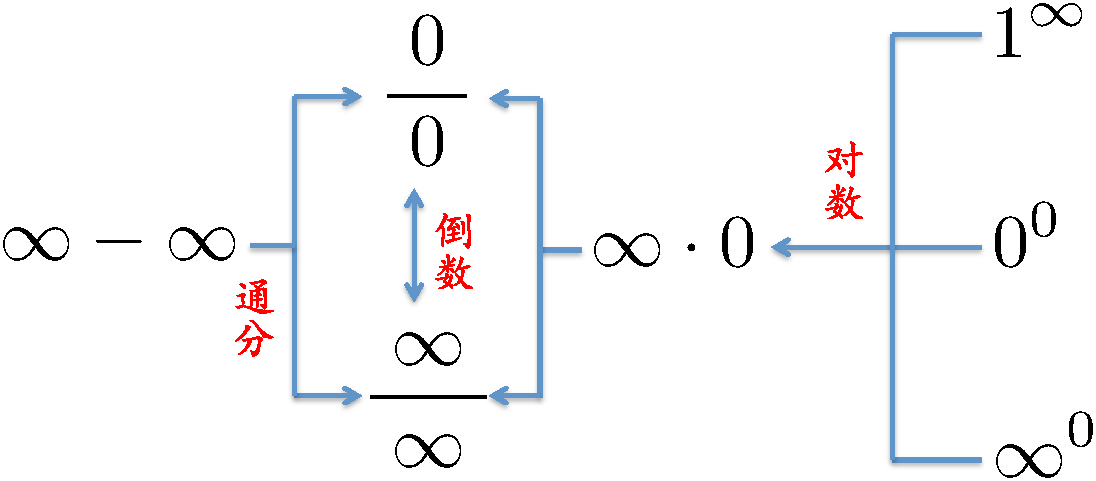
\includegraphics{./images/ch5/lim00.pdf}}
\end{center}

{\bf 习题5.2-15:}设$f(x)$在$x_0$附近存在二阶连续导函数,则
$$\lim\limits_{h\to 0}\df{f(x_0+h)+f(x_0-h)-2f(x_0)}{h^2}=f\,''(x_0).$$
若条件减弱为“$f(x)$在$x=x_0$处二阶可导”,结论是否仍然成立?

{\bf 例:}
设$f(0)=1$,且
$$\limx{0}\df{\ln(1-x)+f(x)\sin x}{e^{x^2}-1}=0,$$
证明:$f(x)$在$x=0$处可导,求$f\,'(0)$。

\section{函数的单调性、凹凸性}

\subsection{可导函数的单调性与极值}

\subsubsection{单调性}

{\bf 定理5.4.1:}设$f(x)$在$[a,b]$上连续,$(a,b)$内可导,且$f\,'(x)$恒大(小)于零,
则$f(x)$在$[a,b]$上严格单调递增(减)。

\begin{itemize}
  \setlength{\itemindent}{1cm}
  \item {以上仅仅是判定可导函数严格单调的充分条件,而非充要条件} 
  \item {若定理中的“大(小)于”改成“大(小)于等于”,则对应于单调递增情形,且为充要条件}
\end{itemize}

{\bf P264-例1-2:}讨论$y=x-\sin x$的单调性。

{\bf 定理}(可导函数单调的充要条件)设$f(x)$在$[a,b]$上连续,$(a,b)$内可导,
则$f(x)$在$[a,b]$上严格单调递增,当且仅当:
\begin{enumerate}[(1)]
  \setlength{\itemindent}{1cm}
  \item $f\,'(x)\geq 0,\;x\in(a,b)$
  \item 在$(a,b)$的任意子区间上$f\,'(x)$不恒为零
\end{enumerate}

{\bf 注:}导函数只有{\it 孤立零点}的函数严格单调

\subsubsection{单调性的应用}

{\bf 推论1:}设$\varphi(x),\psi(x) $均在$[a,b]$上可导,且:
\begin{enumerate}[(1)]
  \setlength{\itemindent}{1cm}
  \item $\varphi'(x)>\psi'(x),\;x\in(a,b)$
  \item $\varphi(a)=\psi(a)$
\end{enumerate}
则在$(a,b)$上,恒有$\varphi(x)>\psi(x)$

{\bf 例:}证明:当$x>0$时,恒有
$$x-\df 16x^3<\sin x<x.$$

{\bf 推论2:}设$\varphi(x),\psi(x) $均在$[a,b]$上{\b $n$阶可导},且:
\begin{enumerate}[(1)]
  \setlength{\itemindent}{1cm}
  \item {\b $\varphi^{(n)}(x)>\psi^{(n)}(x),\;x\in(a,b)$}
  \item {\b $\varphi^{(k)}(a)=\psi^{(k)}(a),k=0,1,2,\ldots,n-1$}
\end{enumerate}
则在$(a,b)$上,恒有$\varphi(x)>\psi(x)$

{\bf 例:}证明下列不等式
\begin{enumerate}[(1)]
  \setlength{\itemindent}{1cm}
  \item $\ln(1+x)>\df{\arctan x}{1+x},\;(x>0)$
  \item $e^x>1+x+\df
  {x^2}{2!}+\df{x^3}{3!}+\ldots+\df{x^n}{n!},\;(x>0,n\in\mathbb{N})$
\end{enumerate}

\subsubsection{可导函数的极值}

{\bf 定理5.4.2}极值第一充分条件)
设$f(x)$在$x_0$连续,在$x_0$的去心领域内可导,且$f\,'(x)$在$x_0$两侧导数值异号,则
$f(x)$在$x_0$处取极值。

{\bf 例:}讨论以下函数的极值
\begin{enumerate}[(1)]
  \setlength{\itemindent}{1cm}
  \item $f(x)=2-|x^3-1|$
  \item $f(x)=\left(1+x+\df{x^2}{2!}+\ldots+\df{x^n}{n!}\right)e^{-x}$ 
\end{enumerate}

{\bf 定理5.4.3}(极值第二充分条件)
设$f(x)$在$x_0$二阶可导,且$f\,'(x_0)=0$,则
\begin{enumerate}[(1)]
  \setlength{\itemindent}{1cm}
  \item 若$f\,''(x_0)<0$,$f(x)$在$x_0$处取极大值 
  \item 若$f\,''(x_0)>0$,$f(x)$在$x_0$处取极小值
\end{enumerate}

{\bf 例:}讨论以下函数的极值
\begin{enumerate}[(1)]
  \setlength{\itemindent}{1cm}
  \item $f(x)=x^3-6x^2+5$\hfill (P267-例4)
  \item $f(x)=\cos x+\df12\cos 2x$
\end{enumerate}

\subsubsection{综合应用}

{\bf 例:}函数$f(x)$对满足
$$xf\,''(x)+3x[f\,'(x)]^2=1-e^{-x}$$
\begin{enumerate}[(1)]
  \setlength{\itemindent}{1cm}
  \item 若$f(x)$在$x=c\ne 0$处有极值,证明其必为极小值;
  \item 若$f(x)$在$x=0$处有极值,该极值为极大还是极小?
\end{enumerate}

{\bf P280-习题7:}求数列$\sqrt[n]n$中最大的一项。

{\bf P270-例7:}判定方程$2^x-2x=1$有几个实根。

{\bf 例:}已知$x>0$时,
$$kx+\df1{x^2}=1$$
有且仅有一个根,求$k$的取值范围。($k<0$或$k=\df29\sqrt 3$)

{\bf 例:}设$f(x)\in C[a,b]$,在$(a,b)$内$f\,''(x)>0$,试讨论
$$F(x)=\df{f(x)-f(a)}{x-a}$$
在$(a,b)$内的单调性。

\subsection{曲线的凹凸性}

{\bf 约定:}以下的凹凸均指“上凹”和“上凸”

{\bf 定义5.4.1:}设函数$f(x)$在区间$I$上有定义,若对任意$x_1,x_2\in I$,
以及任意$\lambda\in[0,1]$,有
$$f[\lambda x_1+(1-\lambda)x_2]\leq\lambda f(x_1)+(1-\lambda)f(x_2)$$
则称$f(x)$是区间$I$上的{\it 凹函数}。若上式中的等号严格成立,则称其为{\it 严格凹函数}。

{\bf 注:}几何特征:任意两点间的割线都不会位于两点间曲线的下方

{\bf 定理5.4.4}(可导凹函数的充要条件)
设$f(x)$在$(a,b)$内可导,则$f(x)$为$(a,b)$内的凹函数,当且仅当:
对任意$x_1,x_2\in(a,b)$,恒有
$$f(x_2)\geq f(x_1)+f\,'(x_1)(x_2-x_1). $$
不等号严格成立时,对应于严格凹函数的情形。

{\bf 注:}{任意点处的切线总位于曲线下方}

{\bf 定理5.4.4}(充分条件)
设$f(x)$在$(a,b)$二阶可导,则
\begin{enumerate}[(1)]
  \setlength{\itemindent}{1cm}
  \item 若$f\,''(x)$恒不小于零,$f(x)$为凹函数
  \item 若$f\,''(x)$恒不大于零,$f(x)$为凸函数
\end{enumerate}

{\bf 注:}两侧$f\,''(x)$反号的点,{\it 拐点}

{\bf 推论}(P276-例11)严格凸(凹)函数的驻点为极值点。

\subsection{分析作图}

{\bf P279-例14:}作出函数$y=\df{x}{1+x^2}$的图形。

\begin{center}
	\resizebox{!}{5cm}{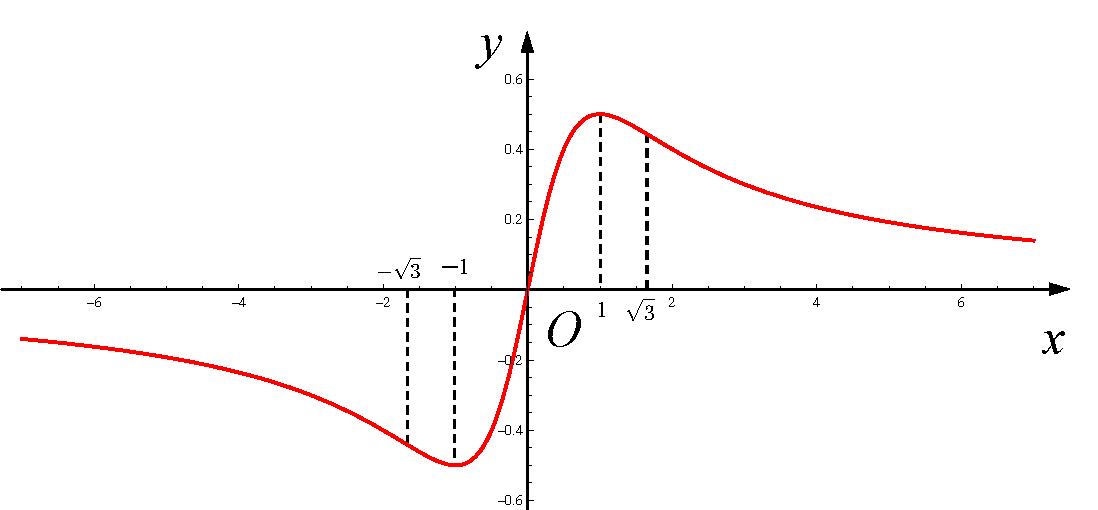
\includegraphics{./images/ch5/x1x2.pdf}}
\end{center}

\begin{shaded}
{\bf 【解题步骤】}
\begin{enumerate}[(1)]
  \setlength{\itemindent}{1cm}
  \item {\bf 分析函数一般性质:}{ 定义域、值域、奇偶性、周期性、与坐标轴的交点}
  \item {\bf 求一、二阶导函数:}{ 确定不可导点}
  \item {\bf 列表分析:}{ 单调、凸凹区间,极值点和拐点}
  \item {\bf 画出渐进线:}{ 水平、铅直和斜渐进线}
  \item {\bf 描点作图}
\end{enumerate}
\end{shaded}

{\bf 例:}函数作图:$y=xe^{1/x}$
\begin{itemize}
  \setlength{\itemindent}{1cm}
  \item 极值点:$y(1)=e$
  \item 渐近线:$y=x+1$
\end{itemize}

\begin{center}
	\resizebox{!}{7cm}{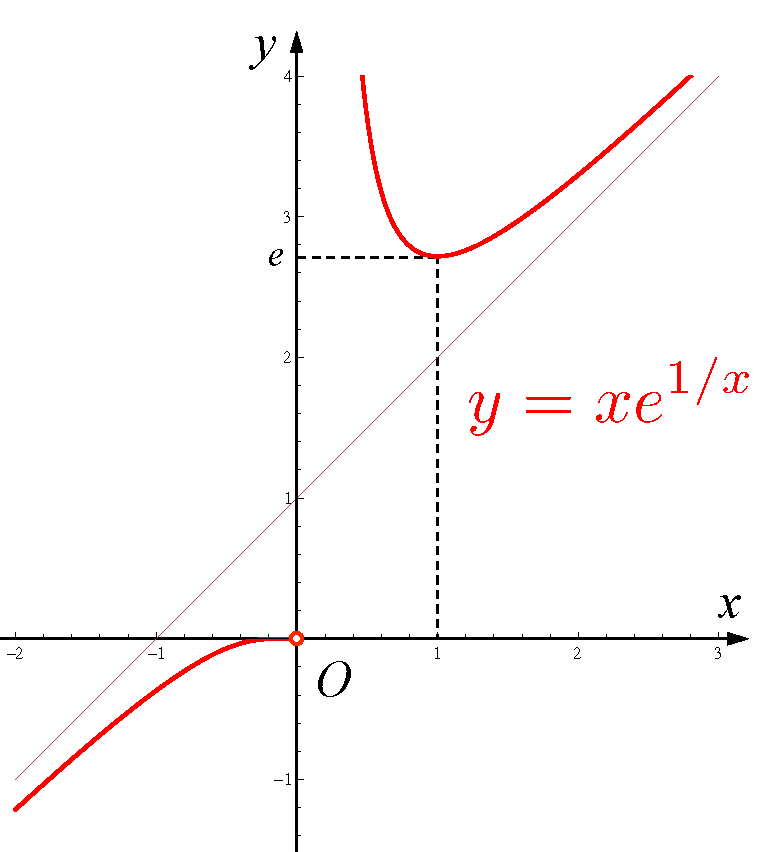
\includegraphics{./images/ch5/xe1x.pdf}}
\end{center}

\section{Taylor公式与函数的多项式逼近}

\subsection{Taylor多项式}

{\bf 定义:}$P(x)$是$f(x)$在点$x_0$处的$n$阶Taylor多项式
\begin{itemize}
  \setlength{\itemindent}{1cm}
  \item $P(x)$是$n$次多项式 
  \item $y=P(x)$在$x_0$处与$y=f(x)$处至少$n$阶相切 
\end{itemize}

$$P_n(x)=\sum\limits_{k=0}^n\df{f^{\,(k)}(x_0)}{k!}(x-x_0)^k$$
\begin{itemize} 
  \item {给定$f(x)$和$x_0$,$P_n(x)$唯一确定} 
  \item 若$x_0=0$,称为{\it $f(x)$的$n$阶Maclaurin多项式}
\end{itemize}

{\bf P248-例1-2:}求Maclaurin多项式
\begin{enumerate}[(1)]
  \setlength{\itemindent}{1cm}
  \item $f(x)=e^x$ 
  $${P_n(x)=1+x+\df{x^2}{2!}+\ldots+\df{x^n}{n!}}$$ 
  \item $f(x)=\cos x$ 
  $${P_n(x)=1-\df{x^2}{2!}+\df{x^4}{4!}-\ldots+(-1)^m\cdot\df{x^{2m}}{(2m)!}}$$
\end{enumerate}

\subsection{误差估计}

{\bf 定理5.3.1:}设函数$f(x)$在$x_0$处$n$阶可导,$P(x)$是$f(x)$在点$x_0$处
的$n$阶Taylor多项式,则当$x\to x_0$时
$${|f(x)-P_n(x)|=\circ[(x-x_0)^n]}$$

\begin{itemize}
  \setlength{\itemindent}{1cm}
  \item {\it 余项:}$R_n(x)=|f(x)-P_n(x)|$ 
  \item {\it 带Peano余项的$n$阶Taylor公式:}
  $${f(x)=P_n(x)+\circ[(x-x_0)^n]}$$
\end{itemize}

{\bf 定理5.3.2}(Taylor中值定理)
设$f(x)$在$x_0$的某领域内$n+1$阶可导,对该领域内任一点$x$,存在介于
$x_0$和$x$之间的一点$\xi$,满足
$${f(x)=P_n(x)+\df{f^{(n+1)}(\xi)}{\,(n+1)!}(x-x_0)^{n+1}}$$
上式称为{\it 带Lagrange余项的$n$阶Taylor公式}
$$f(x_0+h)=P_n(x_0+h)+\df{f^{\,(n+1)}(x_0+\theta
h)}{(n+1)!}h^{n+1},(0<\theta<1)$$

{\bf 推论:}若存在常数$C>0$,使当$x\in(a,b)$时,恒有
$$|f^{\,(n+1)}(x)|\leq C,\;n=0,1,2,\ldots$$
则
$$\limn [f(x)-P_n(x)]=0.$$
也即:Taylor多项式的次数越高,逼近精度越高。

{\bf 例}(常用的Maclaurin公式)
\begin{enumerate}[(1)]
  \setlength{\itemindent}{1cm}
  \item {$e^x =\sum\limits_{k=0}^n\df{x^k}{k!}
  +\df{e^{\theta x}}{(n+1)!}x^{n+1}\;
  (0<\theta<1,x\in\mathbb{R})$}
  \item {$\sin x
  =\sum\limits_{k=1}^m(-1)^{k-1}\df{x^{2k-1}}{(2k-1)!} 
  +(-1)^m\df{\cos\theta x}{(2m+1)!}x^{2m+1}\;
  (0<\theta<1,x\in\mathbb{R})$}
  \item {$\cos x= \sum\limits_{k=0}^m(-1)^{k}\df{x^{2k}}{(2k)!}
  +(-1)^{m+1}\df{\sin\theta
  x}{(2m+2)!}x^{2m+2}\; (0<\theta<1,x\in\mathbb{R})$}
  \item
  {$\ln(1+x) =\sum\limits_{k=1}^n(-1)^{k-1}\df{x^k}{k}
  +\df{(-1)^nx^{n+1}}{(n+1)(1+\theta
  x)^{n+1}}\; (0<\theta<1,x>-1)$} 
  \item
  {$(1+x)^\alpha =\sum\limits_{k=0}^n
  \df{\alpha(\alpha-1)\ldots(\alpha-k+1)}{k!}x^k
	 +\df{\alpha(\alpha-1)\ldots(\alpha-n)}{(n+1)!}\df{x^{n+1}}{(1+\theta
	x)^{n+1-\alpha}}\quad (0<\theta<1,x\ne -1)$}
\end{enumerate}

\subsection{函数的Taylor展开}

{\bf 问题:}{ 给定函数$f(x)$,求其在$x_0$的$n$阶Taylor公式} 
\begin{enumerate}[(1)]
  \setlength{\itemindent}{1cm}
  \item {\bf 直接法(公式法)} 
  \begin{itemize}
    \item 逐个计算Taylor系数,给出相应的公式 
  \end{itemize}
  \item {\bf 间接法} 
  \begin{itemize}
    \item 利用已知函数的Maclaurin公式 
    \item 利用级数和多项式的性质
  \end{itemize}
\end{enumerate}

\subsubsection{多项式函数}

{\bf 定理}
多项式函数$P_n(x)=\sum\limits_{k=0}^na_kx^k$的$m$阶Maclaurin多项式为其$m$次
{\it 截断多项式:} 
$${P_m(x)=\sum\limits_{k=0}^ma_kx^k}$$

{\bf P259-习题1:}求$f(x)=x^3+3x^2-2x+4$的各阶Maclaurin多项式和在
$x=1$处的Taylor多项式。

\subsubsection{直接法求Taylor展开式}

{\bf P254-例3:}求$f(x)=\tan x$的$3$阶带有Peano余项的Maclaurin公式。

\begin{itemize}
  \setlength{\itemindent}{1cm}
  \item 直接法 
  \item 待定系数法
\end{itemize}

\subsubsection{间接法求Taylor展开式}

{\bf 规则一:}若在区间$I$内,$f(x)=\sum\limits_{n=0}^{\infty}a_nx^n$,
$g(x)=\sum\limits_{n=0}^{\infty}b_nx^n$,则
\begin{enumerate}[(1)]
  \setlength{\itemindent}{1cm}
  \item $\lambda f(x)+\mu g(x)=\sum\limits_{n=0}^{\infty}(\lambda a_n+\mu
  b_n)x^n$,其中$\lambda,\mu$为常数 
  \item $f\,'(x)=\sum\limits_{n=0}^{\infty}na_{n}x^{n-1}$ 
  \item $\displaystyle\int f(x)dx=\sum\limits_{n=0}^{\infty}
  \df{a_{n}}{n+1}x^{n+1}$
\end{enumerate}

{\bf  P254-例4:}求$f(x)=\df 12\ln\df{1+x}{1-x}$的$n$阶带有Peano余项的Maclaurin公式。

{\bf P255-例5:}求$f(x)=\df 1{2+x}$在$x=1$处的$7$阶Taylor多项式,并求$f^{(7)}(1)$。

{\bf 规则二:}若在区间$I$上,恒有$f(x)=\sum\limits_{n=1}^{\infty}a_nx^n$,
给定函数$g(x)$,当$g(x)\in I$时,恒有
$$f[g(x)]=\sum\limits_{n=1}^{\infty}a_n[g(x)]^n.$$

{\bf 习题5.3-4:}求带有Peano余项的Maclaurin公式
\begin{enumerate}[(1)]
  \setlength{\itemindent}{1cm}
  \item $f(x)=\ln(2+x)$ 
  \item $f(x)=e^{-x^2}$
  \item $f(x)=x\sin x$ 
  \item $f(x)=\df{x^2}{1+x}$ 
  \item $f(x)=\df{1}{\sqrt{1-x^2}}$ 
  \item $f(x)=\cos^2x$
\end{enumerate}

\subsection{Taylor公式的应用}

\subsubsection{近似计算}

{\bf P256-例6:}计算$e$的值,误差不超过$10^{-5}$。

\begin{center}
	\resizebox{!}{5.5cm}{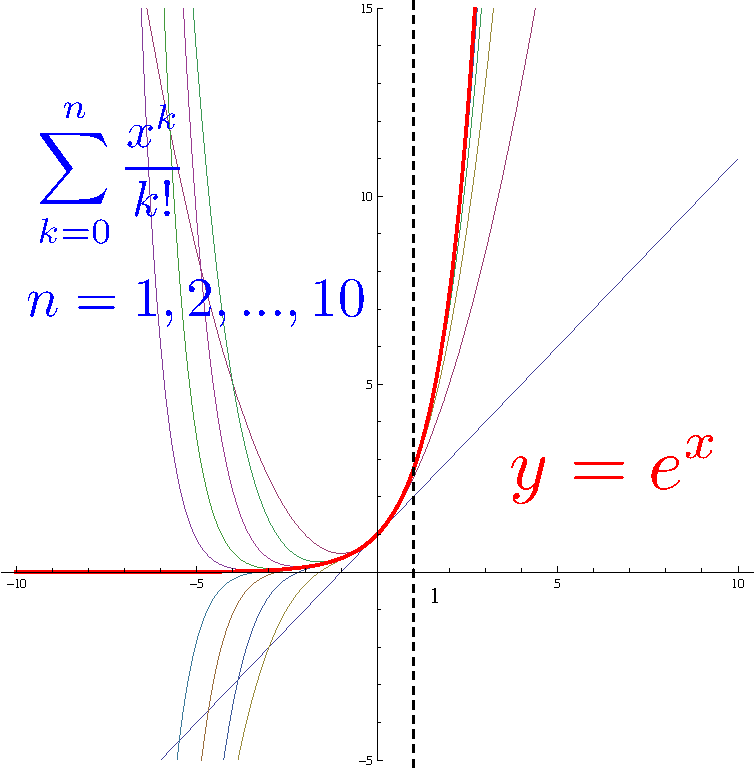
\includegraphics{./images/ch5/exse1.pdf}}\quad
	\resizebox{!}{5.5cm}{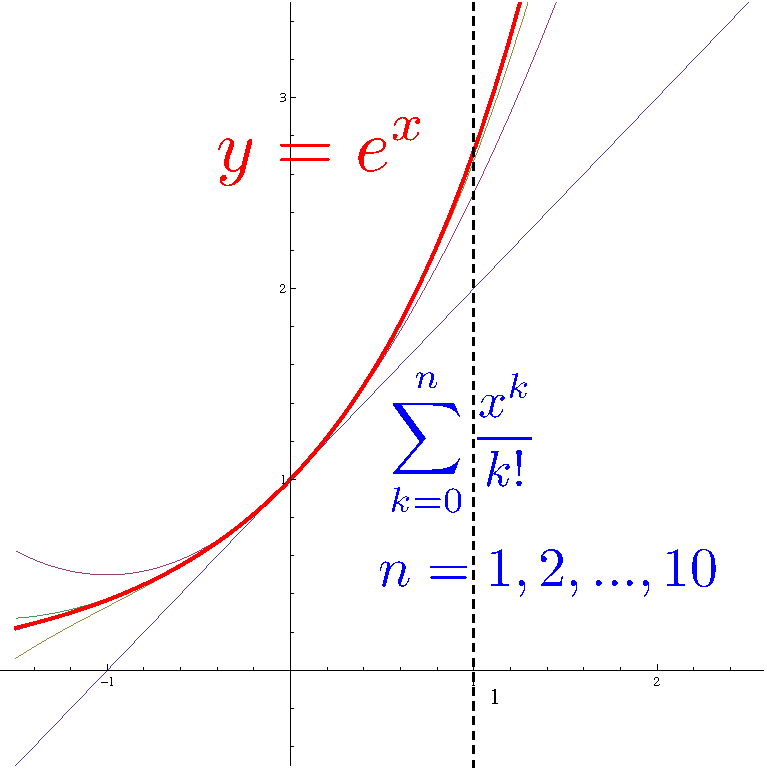
\includegraphics{./images/ch5/exse2.pdf}}
\end{center}

\subsubsection{计算不定式极限}

{\bf P257-例8:}计算以下极限
\begin{enumerate}[(1)]
  \setlength{\itemindent}{1cm}
  \item $\limx{0}\df{\cos x-e^{-x^2/2}}{x^4}$ 
  \item $\limx{0}\df{\tan x-\sin x}{x^3}$
  \item $\limx{0}\df{\df{x^2}{2}+1-\sqrt{1+x^2}}{x^2\sin x^2}$ 
  \item $\limx{0}\df{e^x-1-x}{\df{1}{\sqrt{1-x}}-\cos\sqrt x}$ 
  \item $\limx{0}\df{\cos(\sin x)-\cos x}{x^4}$
  \item $\limx{+\infty}\left[x-x^2\ln\left(1+\df 1x\right)\right]$
\end{enumerate}

{\bf 注:}不知道该展开到多少阶时,先进行试探性展开

{\bf 例:}设$f(x)$在$x=0$附近二次可导,且
$$\limx{0}\left(1+x+\df{f(x)}{x}\right)^{1/x}=e^3,$$
求:
\begin{enumerate}[(1)]
  \setlength{\itemindent}{1cm}
  \item $f(0),f\,'(0),f\,''(0)$;
  \item $\limx{0}\left(1+\df{f(x)}{x}\right)^{1/x}$.
\end{enumerate}

\subsubsection{证明不等式}

{\bf P258-例9:}证明:$x>0$时,$e^x>1+x+\df{x^2}{2}$

{\bf P259-例10:}设$f(x)$在$(a,+\infty)$内具有二阶导数,
且$f(x),f\,''(x)$在$(a,+\infty)$
有界,证明:$f\,'(x)$在$(a,+\infty)$有界。

{\bf 例:}证明:若在$(a,b)$内,$f\,''(x)>0$,则对任意$a<x_1<x_2<b$,恒有
$$f\left(\df{x_1+x_2}{2}\right)<\df{f(x_1)+f(x_2)}{2}.$$

{\bf 思考:}以上结论能否进一步推广?
$${f(\lambda x_1+(1-\lambda)x_2)<\lambda
f(x_1)+(1-\lambda)f(x_2),\;0<\lambda<1}$$

{\bf 例:}设在$f(x)$在$[0,a]$上二阶连续可导,
$|f\,''(x)|\leq M$,且$|f(x)|$在$(0,a)$内可取到最大值,证明:
$$|f\,'(0)+f\,'(a)|\leq Ma.$$

{\bf 例:}设$f(x)$在$[0,1]$上二阶连续可导,且$f(0)=f(1)$, \\
$|f\,''(x)|\leq A$,证明:对任意$x\in[0,1]$,恒有
$$|f\,'(x)|\leq\df A2.$$

{\bf 用Taylor公式证明等式或不等式} 
\begin{itemize}
  \item 多使用Lagrange余项
  \item 特殊的点: 区间端点、 极(最)值点、
  区间中点、 距离为常数的点、 已知条件中提到的特殊点
\end{itemize}

{\bf 辅导书P153-例37:}
设$f(x)$在$[a,b]$上二阶连续可导,且$f\,'(a)=f\,'(b)=0$,则至少存在一点
$c\in(a,b)$,使得
$$|f\,''(c)|\geq \df 4{(b-a)^2}|f(b)-f(a)|.$$

\section{曲率}

{\bf 问题:}如何刻画一条平面曲线的几何特征?

\begin{itemize}
  \setlength{\itemindent}{1cm}
  \item {\bf 切线斜率:}一阶导数
  \item {\bf 凹凸性:}二阶导数
  \item {\bf 长度:}弧微分
  \item {\bf 弯曲程度:}{\b 曲率}
\end{itemize}

\subsection{弧微分}

{\bb 弧微分:}曲线$y=f(x)$的弧长关于自变量$x$的微分 
$$\d s=\sqrt{1+(y')^2}\d x =\sqrt{(\d x)^2+(\d y)^2}$$ 
\begin{itemize}
  \setlength{\itemindent}{1cm}
  \item 参数方程形式 
  $$\d s=\sqrt{[x'(t)]^2+[y'(t)]^2}\d t$$ 
  \vspace{-3ex}
  \item 极坐标形式 
  $$\d s=\sqrt{\rho^2(\theta)+[\rho'(\theta)]^2}\d\theta$$
\end{itemize}

\subsection{曲率}

\begin{center}
	\resizebox{!}{7cm}{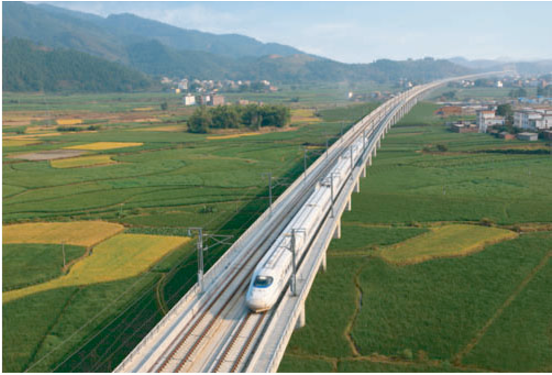
\includegraphics{./images/ch5/rw1.pdf}}
	
	铁路的设计问题
\end{center}

\subsubsection{概念}

{\bf 问题:}如何刻画曲线的弯曲程度?

\begin{center}
	\resizebox{!}{5.5cm}{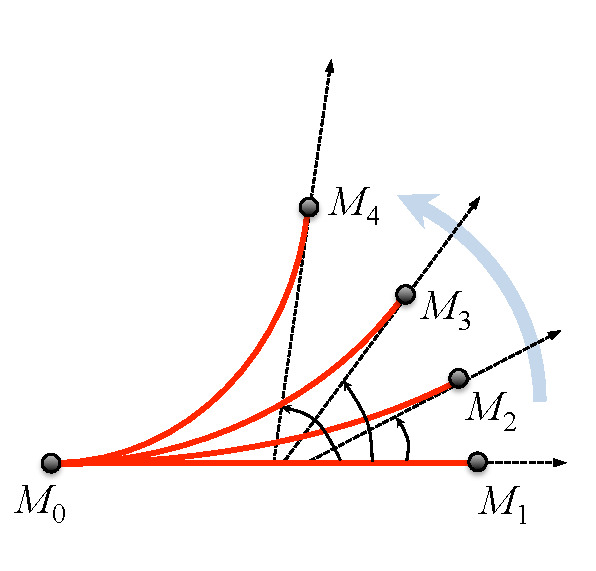
\includegraphics{./images/ch5/curves/c101.pdf}}\quad
	\resizebox{!}{5.5cm}{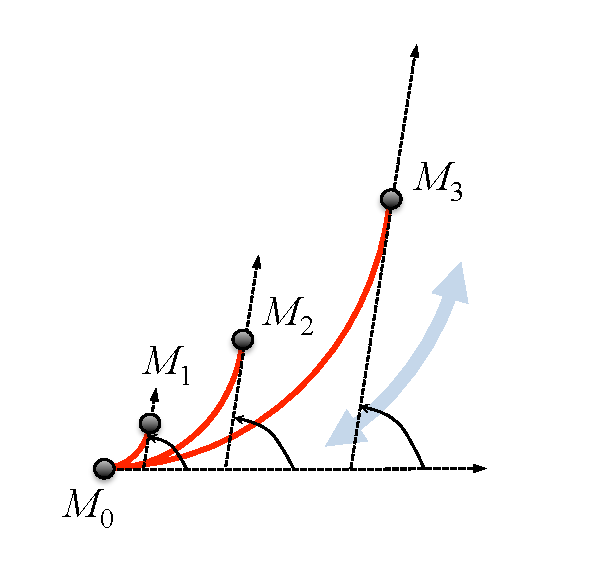
\includegraphics{./images/ch5/curves/c201.pdf}}
\end{center}

\begin{itemize}
  \setlength{\itemindent}{1cm}
  \item 长度相同的曲线,切线转角越大弯曲程度越大
  \item 切线转角相同的曲线,弧长越短弯曲程度越大
\end{itemize}

{\it 曲线的弯曲程度与切线的转角成正比,与弧长成反比}

{\bf 定义5.5.1:}设曲线$C$光滑且可求长度。 从其上一点$M_0$出发,
到另一点$M$的弧长为$\Delta s$,切线转角为$\Delta\alpha$。
 若极限$\lim\limits_{\Delta s\to
0}\left|\df{\Delta\alpha}{\Delta s}\right|$存在,
则称之为{\it 曲线$C$在$M_0$处的曲率:}

$${K=\lim\limits_{\Delta s\to
0}\left|\df{\Delta\alpha}{\Delta s}\right|
=\left|\df{\d\alpha}{\d s}\right|}$$ 

{\bf 曲率:}在曲线上某一点处的切线转角关于弧长的变化率

% $$K=\df{|y''|}{(1+(y')^2)^{\frac32}}$$

设$y=f(x)$在$x_0$的某邻域内二阶可导,则
{$$K=\left|\df{\d\alpha}{\d s}\right|
 =\df{|y''_{xx}|}{[1+(y'_x)^2]^{3/2}}$$}
 
{\bf P286-例2:}求直线与圆的曲率。

{\bf 例:}求椭圆$x=3\cos t,y=2\sin t\,(0\leq t\leq 2\pi)$
上任意点处的曲率,并指出其中曲率最大的点。

\begin{center}
	\resizebox{!}{4.5cm}{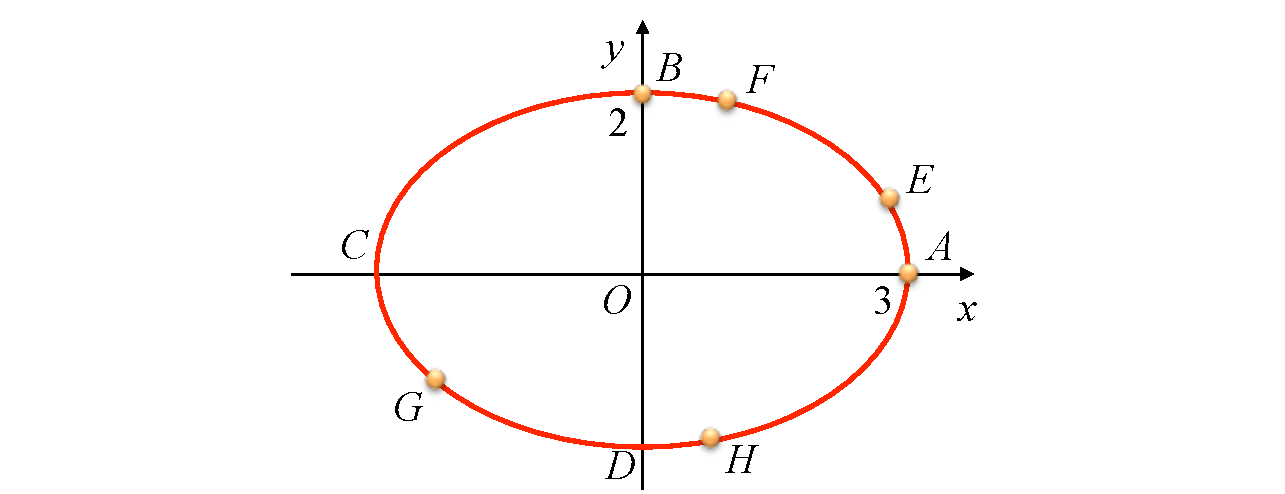
\includegraphics{./images/ch5/ec/newEC/ec01.pdf}}
\end{center}

{\bf 注:} {参数方程下的曲率公式}
$${K=\df{|x'_ty''_{tt}-x''_{tt}y'_t|}
{\{[x'_t]^2+[y'_t]^2\}^{3/2}}}$$

{\bf 思考:}如何给出极坐标下的曲率公式?

\subsubsection{曲率圆与曲率的应用}

{\bf 曲率圆:}与给定曲线在凹侧相切,且曲率相同的圆

\begin{center}
	\resizebox{!}{4cm}{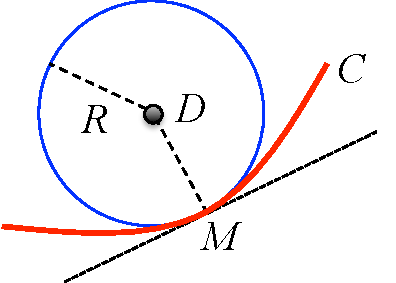
\includegraphics{./images/ch5/curSphere.pdf}}
\end{center}

{\bf 思考:}与已知曲线在给定点处二阶相切的圆一定是其曲率圆吗?(${\bm{\surd}}$)

{\bf 定理:}曲率圆与给定曲线二阶相切。

{\bf 例}(加工问题)已知某工件内侧的截痕曲线为椭圆$\df{x^2}9+\df{y^2}4=1$,
若用圆形砂轮对其进行打磨,问该如何选择砂轮的尺寸?

\begin{center}
	\resizebox{!}{5.5cm}{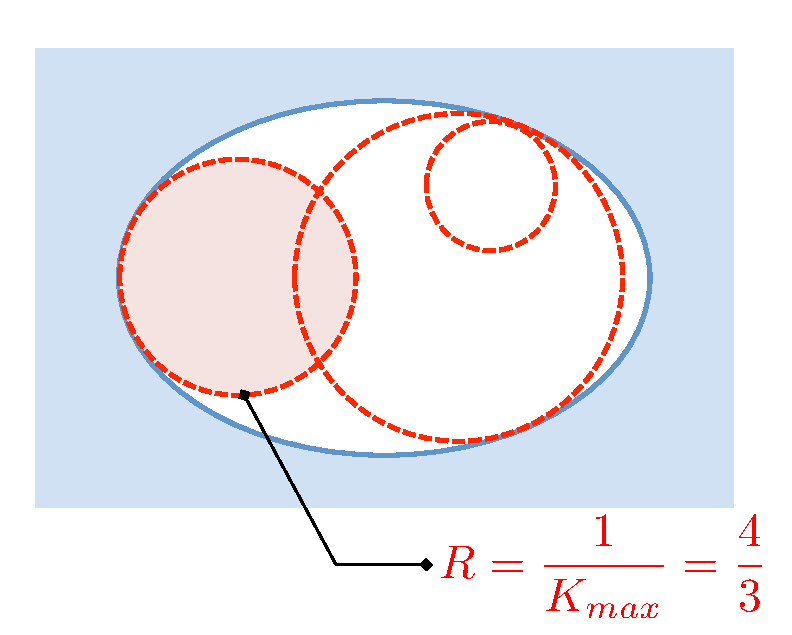
\includegraphics{./images/ch5/SE/S01.pdf}}
\end{center}

{\bf 注:}利用砂轮磨削一般工件的内表面时,砂轮的半径不应超过工件内表面
的截线上各点处的曲率半径的最小值

{\bf 定律:}质量为$m$的质点以速度$v$通过光滑曲线上一点,所受离心力为
$$F=\df{mv^2}{R},$$
其中$R$为曲线在该点处的曲率半径。

\begin{center}
	\resizebox{!}{4.5cm}{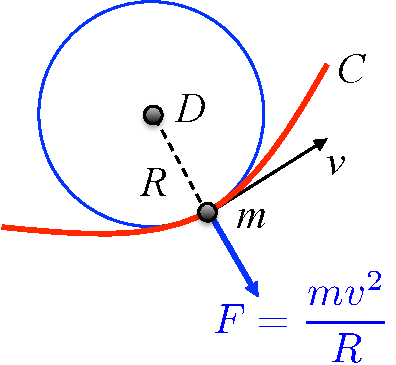
\includegraphics{./images/ch5/flip.pdf}}
\end{center}

\subsubsection{铁路中的缓和曲线}

\begin{center}
	\resizebox{!}{4.5cm}{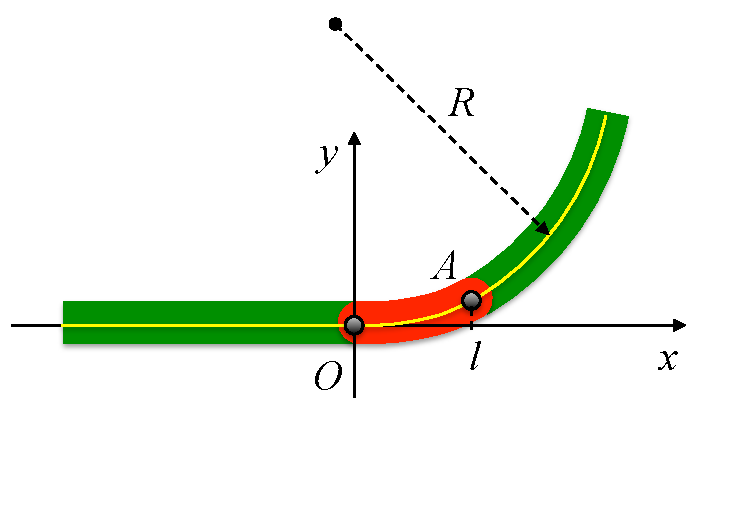
\includegraphics{./images/ch5/rc02.pdf}}
\end{center}

{\bf 设计要求:}为了确保列车行驶安全,尽可能保证列车运行时所受离心力的平稳变化

{\bf 常用的缓和曲线:}

\begin{itemize}
  \setlength{\itemindent}{1cm}
  \item {三次多项式}
  \item {渐开螺旋线}
  \item {双纽线}
  \item {\ldots}
\end{itemize}

{\bf 例:}如图,列车匀速行进,经过一段直线轨道后,将进入半径为$R$的圆弧轨道。为
尽量减少列车行驶中所受的离心力冲击,试确定一个三次多项式函数实现两段轨道的连接。

\begin{center}
	\resizebox{!}{5.2cm}{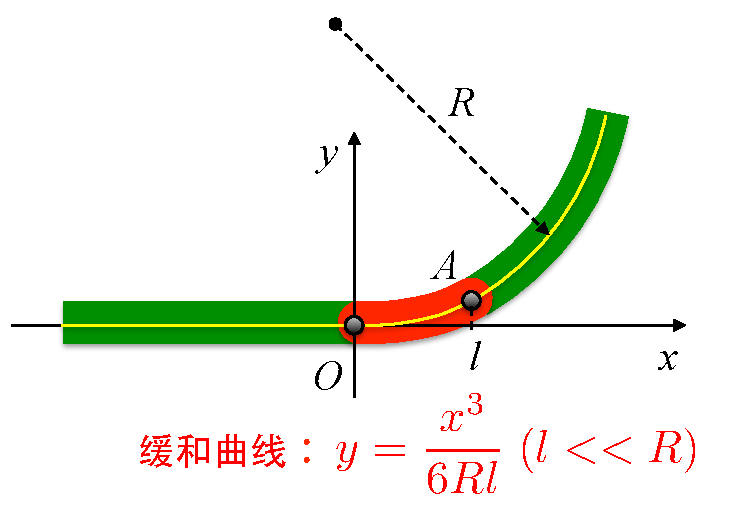
\includegraphics{./images/ch5/rc01.pdf}}
\end{center}

\begin{itemize}
  \item 匀速行驶$v=108km/h$
  \item 列车重量$m=500t$
  \item 圆弧半径$R=1000m$
  \item 缓和曲线长$l=90m$
\end{itemize}

\begin{center}
	\resizebox{!}{4cm}{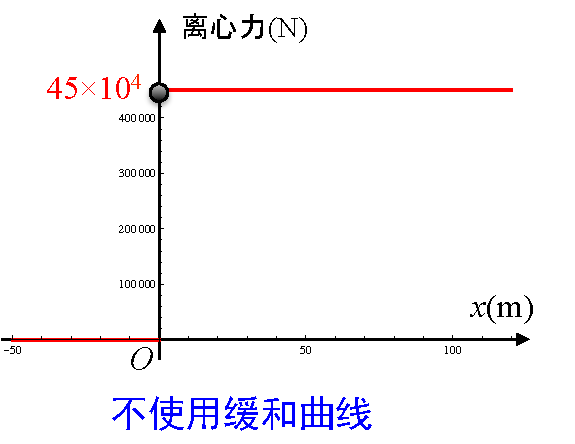
\includegraphics{./images/ch5/f01.pdf}}\quad
	\resizebox{!}{4cm}{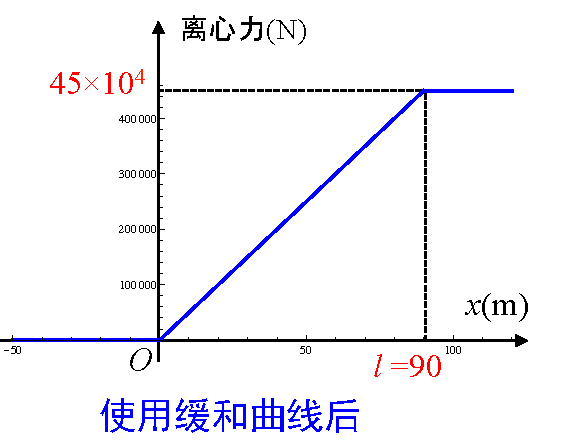
\includegraphics{./images/ch5/f02.pdf}}
\end{center}

类似的问题广泛存在于高速公路、过山车,甚至是飞行器表面的设计中。

\newpage

\section*{习题与课后思考题}

\section*{课后作业}

\begin{itemize}
  \item 习题5.1:5,6,7,9,12,14
  \item 习题5.2:3,7,9,11,14,17
  \item 习题5.3:2,4,6,10(2,4),13,16
  \item 习题3.3:10
  \item 习题5.4:6(2,4),8,9(1),10,11,12,13,14(3)
  \item 习题5.5:5,6,7,8,11
\end{itemize}

{\bf 【课堂练习与思考题】}

\begin{itemize}
  \item 习题5.1:10,11,13
  \item 习题5.2:2,5,8,10,12,13,15,16,18
  \item 习题5.3:1,5,8,9,12,14
  \item 计算如下极限
  	\begin{enumerate}
	  \item $\limx{0}\df{e^x-e^{-x}-2x}{x-\sin x}$ 
	  \item $\limx{0}\df{e^{-1/x^2}}{x^{100}}$ 
	  \item $\limx{a}\df{x^a-a^x}{x^x-a^a}\;(a>0)$ 
	  \item $\limx{0}\left(\df{a^x+b^x+c^x}{3}\right)^{1/x}$ 
	  \item $\limn\sqrt{n}(\sqrt[n]{n}-1)$ 
	  \item $\limn\left(n\sin\df{1}{n}\right)^{n^2}$
	\end{enumerate}	
  \item 习题5.4:4,5,12
  \item (过山车设计)试设计一个分段的多项式函数,完成过山车上两段不同斜率的直线轨道的接合。
\end{itemize}